
\documentclass[a4paper,11pt]{article}

%\usepackage{marvosym}
\usepackage{amsmath}
\usepackage{amssymb}
\usepackage{verbatim}
\usepackage{graphicx}
\usepackage{psfrag}
\usepackage{listings}
\usepackage{booktabs}
\usepackage{caption}
\usepackage{subcaption}

% MARGIN SETTINGS
\setlength{\voffset}{-1.1in}
\setlength{\textheight}{740pt}
%\setlength{\topmargin}{-0.5in}
\setlength{\textwidth}{6.2in}
\setlength{\oddsidemargin}{0.1in}
\setlength{\evensidemargin}{0in}
\setlength{\footskip}{20pt}

\author{Will Booker}
\title{Compressible Acoustic Waves}

\begin{document}

\maketitle

\section{Preliminaries}


A Hamiltonian formulation is a system with either an finite or infinite number of degrees of freedom with a specified structure. The system's dynamics are then described in phase-space using two geometric objects: a total energy functional,  the Hamiltonian $\mathcal{H}$, and a skew symmetric Poisson bracket $\{ , \}$.
As systems of fluid dynamics are continuous in space, we will be considering infinite dimensional dynamical systems. 



 We now consider the general state of a functional $\mathcal{F}$ for  the system in consideration, the functional's time evolution is now described by the following equation,

\begin{equation}
 \frac{ d \mathcal{F}}{dt} =\{\mathcal{F},\mathcal{H}\} .
\end{equation}
The Poisson bracket has to satisfy the following conditions :

\begin{itemize}
\item skew-symmetry: $\{\mathcal{F},\mathcal{H}\}$ = $-\{\mathcal{H},\mathcal{F}\}$,
\item linearity: $\{\alpha \mathcal{F} + \beta \mathcal{G},\mathcal{H}\}$ = $\alpha \{\mathcal{F},\mathcal{H}\}$ + $\beta\{\mathcal{G},\mathcal{H}\}$,
\item Jacobi identity: $ \{\mathcal{F},\{\mathcal{G},\mathcal{H}\}\}$ + $ \{\mathcal{G},\{\mathcal{H},\mathcal{F}\}\}$ + $ \{\mathcal{H},\{\mathcal{F},\mathcal{G}\}\}$ = 0,
\item Leibniz identity:   $\{\mathcal{F}\mathcal{G},\mathcal{H}\}$ = $\mathcal{F}\{\mathcal{G},\mathcal{H}\}$ + $\{\mathcal{F},\mathcal{H}\}\mathcal{G}$,
\end{itemize}
where $\alpha$, $\beta$ are constants, and $\mathcal{F}$, $\mathcal{G}$, $\mathcal{H}$ are arbitrary functionals. \\
We  note that the skew-symmetry condition automatically yields energy conservation for the system,
\[\frac{d \mathcal{H}}{dt} = \{\mathcal{H},\mathcal{H}\}= -\{\mathcal{H},\mathcal{H}\} = 0.\]
We first  need to define a variational derivative, 
\begin{equation}\label{eqns:var_deriv}
\delta \mathcal{H} = \lim_{\epsilon \rightarrow 0}\frac{ \mathcal{H}( u+ \epsilon\delta u)-  \mathcal{H}(u)}{\epsilon}= \bigg ( \frac{\delta  \mathcal{H}}{\delta u}, \delta u \bigg)+  \mathcal{O}(\delta u^2),
\end{equation}
where $(\cdot,\cdot)$ is the inner product for the function space $\{ u\}$.



\section{Continuum Description}

In this report we will consider in a compressible fluid in a three-dimensional domain $\Omega$ . We will assume that viscous effects and temperature effects do not influence the motion of the fluid. We assume that the resting density, $\rho_0$ and acoustic speed of sound $c^2_0$ have been scaled such that $\rho_0$ =  $c^2_0$ = 1  , and that the  equations of motions  have been linearised around a state of rest. This leads to the linear compressible Euler equations

\begin{equation}\label{eqns:euler}
\begin{aligned}
\frac{\partial \mathbf{u}  }{\partial t} &= -\nabla \rho ,\\
\frac{\partial \rho }{\partial t} &= - \nabla \cdot \mathbf{u} .
\end{aligned}
\end{equation}

We will take that $\partial \Omega$ i.e. the boundary of our considered domain is  taken to be solid walls, such that there is no normal flow through them. 

\[ \hat{\underline{n}}.\cdot \mathbf{u}= 0 \text{ on } \partial \Omega .\]




Hamiltonian dynamics of compressible fluid flow governed by equations \eqref{eqns:euler} is given by

\begin{equation}\label{eqns:pb} \{ \mathcal{F},  \mathcal{H}\} = \int_\Omega \frac{\delta  \mathcal{H}}{\delta \rho} \nabla \cdot \frac{\delta  \mathcal{F}}{\delta \mathbf{u}} - \frac{\delta  \mathcal{F}}{\delta \rho} \nabla \cdot \frac{\delta  \mathcal{H}}{\delta \mathbf{u}} \text{ d}x,\end{equation}
with its associated Hamiltonian energy functional
\[  \mathcal{H} = \int_\Omega \frac{1}{2} ( \mathbf{u}\cdot \mathbf{u} + \rho^2) \text{ d}x.\]
By using equation \eqref{eqns:var_deriv} we can show  that the variational derivatives for our associated Hamiltonian are

\begin{equation}
\frac{\delta \mathcal{H}}{\delta \rho} =\rho, \quad
\frac{\delta \mathcal{H}}{\delta \mathbf{u}}= \mathbf{u}.
\end{equation}

We will now show an equivalence between the Hamiltonian and the PDE representation of compressible fluid flow, by showing how to obtain the continuity equation from the Hamiltonian representation. We define the following functional for the density

\[\mathcal{F}_\rho = \int_\Omega \rho (x,t) \Phi (x) \text{ d}x,\]
 where $\Phi$ $\in$ $\mathcal{N}$ is an arbitrary test function in the following square integrable function space
\[\mathcal{N} = \{ \Phi \in L^2(\Omega) \} \].

The continuity equation can be derived  by using the density functional along with its corresponding functional derivative in the bracket formulation \eqref{eqns:pb}.  We use that the domain in consideration, $\Omega$,  is fixed allowing us to interchange the  integral over the domain and the time derivative, 
\begin{equation}\label{functionalsderivs}
\begin{aligned}
\frac{d \mathcal{F}_\rho}{dt} &= \{\mathcal{F}_\rho, \mathcal{H} \},\\
\int_\Omega \frac{d}{dt}(\rho (x,t)  \Phi (x  ) \text{ d}x&=\int_\Omega - \nabla \cdot \mathbf{u} \Phi \text{ d}x,\\
\int_\Omega \frac{\partial \rho}{\partial t}\Phi  \text{ d}x&= \int_\Omega -\nabla \cdot \mathbf{u} \Phi \text{ d}x.
\end{aligned}
\end{equation}
As the choice of test function was arbitrary, this relationship holds for any $\Phi$ and thus we can derive the continuity equation  from equation \eqref{eqns:euler},
\begin{equation}
 \frac{\partial \rho}{\partial t} = - \nabla \cdot \mathbf{u}.
\end{equation}


\section{ Discrete Description}

 We now approximate the physical domain $\Omega$ with the computational domain $\Omega_h$, which consists of $e$ non-overlapping elements. The set of all edges in the computational domain is $\Gamma$, which consists of interior edges, $\partial e $ and edges which lie on the domain boundary $\partial \Omega$. We introduce discrete variable $\rho_h$ and $\mathbf{u}_h$, which are approximations to their continuous counterparts. The Poisson bracket \eqref{eqns:pb} now becomes discrete

\[ \{  \{ \mathcal{F},  \mathcal{H}\} = \int_\Omega \frac{\delta  \mathcal{H}}{\delta \rho} \nabla \cdot \frac{\delta  \mathcal{F}}{\delta \mathbf{u}} - \frac{\delta  \mathcal{F}}{\delta \rho} \nabla \cdot \frac{\delta  \mathcal{H}}{\delta \mathbf{u}} \text{ d}e.\]

 We integrate the  Poisson bracket by parts and introduce a numerical flux to create a connection between neighbouring elements,

\begin{equation}
\begin{aligned}
 \{ \mathcal{F},  \mathcal{H}\} = & \sum_e \int_e - \nabla \frac{\delta  \mathcal{H}}{\delta \rho_h}\cdot \frac{\delta  \mathcal{F}}{\delta \mathbf{u}_h} + \nabla \frac{\delta  \mathcal{F}}{\delta \rho_h}\cdot \frac{\delta  \mathcal{H}}{\delta \mathbf{u}_h} \text{ d}e \\
 &+ \sum_e \int_{\partial e }  \frac{\delta  \mathcal{H}}{\delta \rho_h}\hat{\underline{n}} \cdot \widehat{\frac{\delta  \mathcal{F}}{\delta \mathbf{u}_h}} - \frac{\delta  \mathcal{F}}{\delta \rho_h}\hat{\underline{n}} \cdot \widehat{\frac{\delta  \mathcal{H}}{\delta \mathbf{u}_h}} \text{ d} S. 
 \end{aligned}
 \end{equation}
 Wide hats on expressions in the boundary integrals indicate terms which will be approximated by numerical fluxes. 
  The  following numerical fluxes are chosen to approximate wide hat terms, where $-$  and $+$ indicate traces from the left and right elements connected to the face
 \begin{equation}
 \begin{aligned}
  \widehat{\frac{\delta  \mathcal{F}}{\delta \mathbf{u}_h}} &= (1-\theta) \frac{\delta  \mathcal{F}}{\delta \mathbf{u}_h^-}+ \theta\frac{\delta  \mathcal{F}}{\delta \mathbf{u}_h^+},  \\
 \widehat{\frac{\delta  \mathcal{H}}{\delta \mathbf{u}_h}}&= (1-\theta) \frac{\delta  \mathcal{H}}{\delta \mathbf{u}_h^-}+ \theta\frac{\delta  \mathcal{H}}{\delta \mathbf{u}_h^+} ,
 \end{aligned}
 \end{equation}
 we will emphasis here that this choice of numerical flux was made to preserve the skew-symmetry of the Poisson bracket.  We note that by summing these interior boundary integrals over each element, they contribute twice to the Poisson bracket. Thus the contribution over each element can be rewritten to a summation over each interior boundary. We also now split contributions from $\Gamma$ into contributions from interior edges and boundary edges
 \begin{equation}
\begin{aligned}
 \{ \mathcal{F},  \mathcal{H}\} = &  \sum_e \int_e - \nabla \frac{\delta  \mathcal{H}}{\delta \rho_h}\cdot \frac{\delta  \mathcal{F}}{\delta \mathbf{u}_h} + \nabla \frac{\delta  \mathcal{F}}{\delta \rho_h}\cdot \frac{\delta  \mathcal{H}}{\delta \mathbf{u}_h} \text{ d}e \\
 &+ \sum_{\partial e} \int_{\partial e } \bigg(  \frac{\delta  \mathcal{H}}{\delta \rho_h^-} -\frac{\delta  \mathcal{H}}{\delta \rho_h^+}\bigg)\hat{\underline{n}} \cdot\bigg ( (1-\theta) \frac{\delta  \mathcal{F}}{\delta  \mathbf{u}_h^-}+ \theta\frac{\delta  \mathcal{F}}{\delta  \mathbf{u}_h^+} \bigg)\\
 & - \bigg(  \frac{\delta  \mathcal{F}}{\delta \rho_h^-} -\frac{\delta  \mathcal{F}}{\delta \rho_h^+}\bigg)\hat{\underline{n}} \cdot\bigg ( (1-\theta) \frac{\delta  \mathcal{H}}{\delta  \mathbf{u}_h^-}+ \theta\frac{\delta  \mathcal{H}}{\delta  \mathbf{u}_h^+} \bigg) \text{ d} \Gamma \\
 &+ \sum_{\partial \Omega} \int_{\partial \Omega_h } \bigg(  \frac{\delta  \mathcal{H}}{\delta \rho_h^-} -\frac{\delta  \mathcal{H}}{\delta \rho_h^+}\bigg)\hat{\underline{n}} \cdot\bigg (   \widehat{\frac{\delta  \mathcal{F}}{\delta  \mathbf{u}_h}} \bigg)\\
 & - \bigg(  \frac{\delta  \mathcal{F}}{\delta \rho_h^-} -\frac{\delta  \mathcal{F}}{\delta \rho_h^+}\bigg)\hat{\underline{n}} \cdot\bigg (   \widehat{\frac{\delta  \mathcal{H}}{\delta  \mathbf{u}_h}} \bigg) \text{ d}  \Gamma
 \end{aligned}
 \end{equation}
 
 At our boundary edges we have solid wall boundaries and thus we have that 
\[\hat{\underline{n}} \cdot \mathbf{u}_h = 0 \implies  \hat{\underline{n}} \cdot \frac{\delta  \mathcal{H}}{\delta \mathbf{u}_h}= 0 \implies  \hat{\underline{n}} \cdot \widehat{\frac{\delta  \mathcal{H}}{\delta \mathbf{u}_h}} = 0.\]
However to preserve the skew symmetry of the bracket, we also require the flux on the test function $  \widehat{\frac{\delta  \mathcal{F}}{\delta u_h}}$ to vanish at these boundaries. Thus in our Poisson bracket we only have surface integral contributions from interior edges, and none from boundary edges.
 This simplifies the Poisson bracket to 
 \begin{equation}\label{eqns:discretepb}
\begin{aligned}
\frac{dF}{dt} =  \{ \mathcal{F},  \mathcal{H}\} = &  \sum_e \int_e - \nabla \frac{\delta  \mathcal{H}}{\delta \rho_h}\cdot \frac{\delta  \mathcal{F}}{\delta \mathbf{u}_h} + \nabla \frac{\delta  \mathcal{F}}{\delta \rho_h}\cdot \frac{\delta  \mathcal{H}}{\delta \mathbf{u}_h} \text{ d}e \\
 &+ \sum_{\partial e} \int_{\partial e } \bigg(  \frac{\delta  \mathcal{H}}{\delta \rho_h^-} -\frac{\delta  \mathcal{H}}{\delta \rho_h^+}\bigg)\hat{\underline{n}} \cdot\bigg ( (1-\theta) \frac{\delta  \mathcal{F}}{\delta  \mathbf{u}_h^-}+ \theta\frac{\delta  \mathcal{F}}{\delta  \mathbf{u}_h^+} \bigg)\\
 & - \bigg(  \frac{\delta  \mathcal{F}}{\delta \rho_h^-} -\frac{\delta  \mathcal{F}}{\delta \rho_h^+}\bigg)\hat{\underline{n}} \cdot\bigg ( (1-\theta) \frac{\delta  \mathcal{H}}{\delta  \mathbf{u}_h^-}+ \theta\frac{\delta  \mathcal{H}}{\delta  \mathbf{u}_h^+} \bigg) \text{ d} \Gamma 
 \end{aligned}
 \end{equation}



\section{Timestepper}
\subsection{Implicit Midpoint rule}
An implicit midpoint rule is used, as it is a known property that the scheme preserves any property of the underlying ODE upto a quadratic order. This will be sufficient for our scheme to preserve its conservation of energy.

\begin{equation} \begin{aligned} \dot {y} &= f(x,y),\\
\frac{y^{n+1}- y^n}{\Delta t} &= \frac{ f(x^{n+1}, y^{n+1}) + f(x^n, y^n)}{2}, \end{aligned}\end{equation}


\section{Firedrake form}

In Firedrake, the user specifies the problem by inputing a space-continuous weak form that governs the problem. For compressible acoustic waves, equation \eqref{eqns:discretepb} is our space continuous weak form. For linear problems, the weak form is inputted in the following form for general test function $v$ and trial function $u$,
\[ a(u,v) = L(v).\]
Here $L$ is taken to be a vector of all known information, as our problem is unsteady $L$ will include information from the previous timestep. $a$ is taken to be the vector of unknown information of unknown information. As our timestepper in consideration is an implicit midpoint rule, the two parts of the linear system can be built as follows

\[ a = F^{n+1} - \frac{\Delta t}{2} \{ F^{n+1} , H\} ,\]
\[ L = F^{n} + \frac{\Delta t}{2} \{ F^{n} , H\}. \]

The code found with this documentation will follow this same notation, we note that the forms for $a$ and $L$ will be split up into small sums. However we will group terms together as skew-symmetric counterparts, to make the code resemble the mathematical notation. 

\subsection{One -dimensional verification}

As our test problem, similar to the MATLAB application, we will consider $\Omega$ = $[0,1]$. 
By seeking a harmonic wave solution to \eqref{eqns:euler} in our test domain, one can show that a solution is 
\begin{equation*}
\begin{aligned}
u &=  \sin(2\pi x )\sin(2\pi(t+\frac{1}{8})),\\
\rho &=  \cos(2\pi x) \cos(2\pi (t + \frac{1}{8})),
\end{aligned}
\end{equation*}
where a phase shift of $\frac{1}{8}$ has been introduced to ensure a non-zero solution at the initial time. We will use this analytic solution to verify our numerical model and to provide our initial condition for the fluid's velocity and density.

\textbf{ Need to mention the following in the derivation:} 
\begin{itemize}
\item We define the variational derivatives before the bilinear form, so that the code for $ a = L$ matches the form of equation \eqref{eqns:discretepb}.
\item Could include some writeup about mixed function space usage.
\item If so, additional mention of the vector function space would make sense.
\item Highlight the difference between the use of split() and .split()
\item While currently not working, initial energy does match MATLAB energy.
\item This means this is worked out  wrong in the stratified case or the initial condition is wrong.
\end{itemize}


\begin{figure}
    \centering
    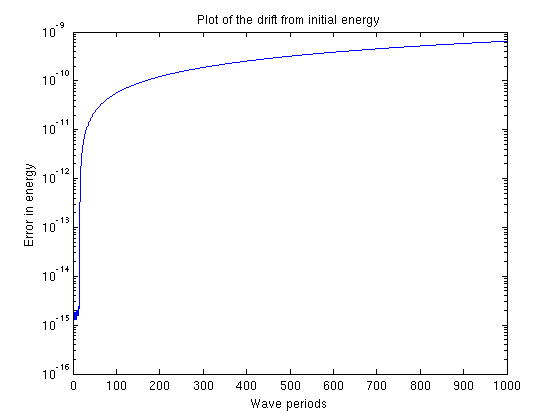
\includegraphics[width=0.75\textwidth]{error1dfd.png}
       \caption{Graphs of the conserved energy for the one-dimensional harmonic wave in Firedrake. The numerical solution was ran for 1000 wave periods. Spatial and temporal  discretisation were set to be 1 / 16. The basis was order 0.}
        \label{test}
\end{figure}


\begin{figure}
    \centering
    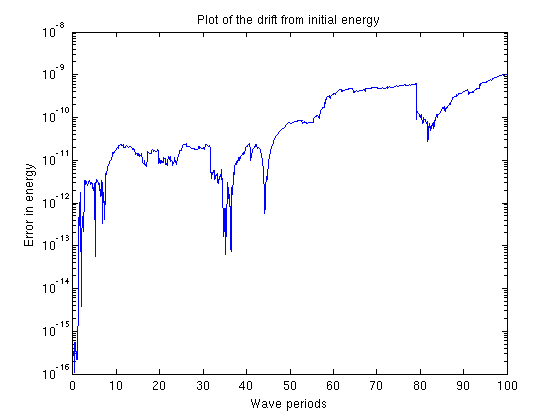
\includegraphics[width=0.75\textwidth]{error1dfdbasis2.png}
       \caption{Graphs of the conserved energy for the one-dimensional harmonic wave in Firedrake. The numerical solution was ran for 100 wave periods. Spatial and temporal  discretisation were set to be 1 / 16. The basis was order 2.}
        \label{test}
\end{figure}



\subsection{Two dimensional verification}

We will now consider the two-dimensional domain  $\Omega$ = $[0,1] \times [0,1]$. We seek again a harmonic wave solution, which yields the following analytic solution for the compressible Euler equations
\begin{equation*}
\begin{aligned}
u &=  \sin(2\pi x )\sin(2\pi(t+\frac{1}{8})),\\
v &=  \sin(2\pi y )\sin(2\pi(t+\frac{1}{8})),\\
\rho &=  \bigg (\cos(2\pi x) +\cos(2\pi y) \bigg ) \cos(2\pi (t + \frac{1}{8})).
\end{aligned}
\end{equation*}
Due to the use of a VectorFunctionSpace in Firedrake, extending the existing one-dimensional code to a two-dimensional problem is now fairly simple. 
The following lines about the mesh and initial condition are changed to be the following


\begin{figure}
    \centering
    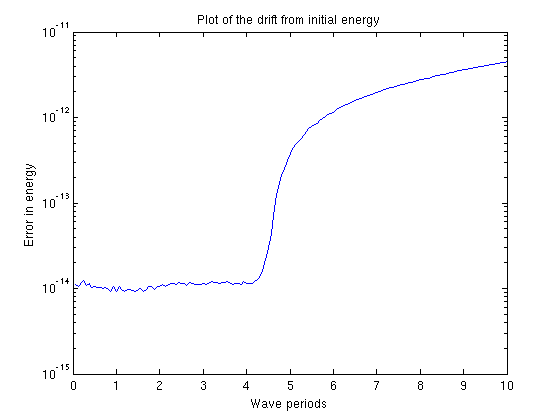
\includegraphics[width=0.75\textwidth]{error2dfd.png}
       \caption{Graphs of the conserved energy for the two-dimensional harmonic wave in Firedrake. The numerical solution was ran for 10 wave periods. Spatial and temporal  discretisation were set to be 1 / 16. The basis was order 0.}
        \label{test}
\end{figure}


\end{document}